%!TEX options=--shell-escape
	\documentclass{article}
	\usepackage{amsmath,amssymb}
	\usepackage[inline]{enumitem}
	\usepackage{blindtext}
	\usepackage{booktabs}
	\usepackage{graphicx}
	\usepackage{xcolor}
	\usepackage[vmargin = 1.5in, top = 1in, bottom = 1.2in, letterpaper]{geometry}
	\usepackage{listings}
	\usepackage{courier}
	\usepackage{multicol}
	\usepackage{multirow}
	\usepackage{bm}
	\usepackage{subcaption}
	\usepackage{minted}
	\usepackage{longtable}
	% \definecolor{bg}{rgb}{0.1,0.1,0.1}
	% \newminted{r}{mathescape, breaklines, linenos = true, bgcolor = bg, formatcom=\color{white}}
	% \usemintedstyle{monokai}
	\definecolor{bg}{rgb}{0.95,0.95,0.95}
	\newminted{r}{mathescape, breaklines, linenos = false, bgcolor = bg}
	\newmintedfile{r}{mathescape, breaklines, linenos = false, bgcolor = bg}
	\usemintedstyle{tango}
	% \lstset{
	% basicstyle = \small\tt,
	% keywordstyle = \tt\color{blue},
	% commentstyle = \it\color[cmyk]{1,0,1,0},
	% stringstyle = \tt\color[RGB]{128,0,0},
	% %frame = single,
	% backgroundcolor = \color[RGB]{245,245,244},
	% breaklines,
	% extendedchars = false,
	% xleftmargin = 2em,
	% xrightmargin = 2em,
	% aboveskip = 1em,
	% tabsize = 4,
	% showspaces = false
	% }
	\newcommand\inner[2]{\left\langle{#1},{#2}\right\rangle}
	\DeclareMathOperator{\Corr}{Corr}
	\DeclareMathOperator{\Cov}{Cov}
	\DeclareMathOperator{\Var}{Var}
	\DeclareMathOperator{\E}{E}



	\begin{document}
	
	% \newfontfamily\courier{Courier New}

	
	\title{STAT 601 Exam 1}
	\author{Yifan Zhu}
	\maketitle
For each of the 4 models, we calculated the marginal expectation, marginal variance and autocorrelation. Here we use autocorrelation to examine the dependence of variables and see if it is decreasing as a function of time separation.
\begin{enumerate}
	\item Model 1.

	For Model 1, we have
	\begin{align*}
	\mu(t) & = \lambda + \gamma[\mu(t-1) - \lambda]\\
	W(t) & = \epsilon_t
	\end{align*}
	and $\mu(0) \sim N(\lambda, \tau^2),\, \epsilon_t \sim N(0, \sigma^2)$.
	Let $\alpha(t) = \mu(t) - \lambda$, then we have
	\[\alpha(t) = \gamma \alpha(t-1)\]
	and $\alpha(0) \sim N(0, \tau^2)$. Then
	\begin{align*}
	\E(Y(t)) &= \E(\mu(t) + W(t)) \\
	&= \E(\mu(t)) = \E(\alpha(t) + \lambda) \\
	&= \lambda + \E(\alpha(t)) \\
	&= \lambda + \E(\gamma \alpha(t-1)) \\
	& = \lambda + \gamma \E(\alpha(t-1))\\
	&= \cdots \\
	&= \lambda + \gamma^t \E(\alpha(0)) \\
	& \lambda + \gamma^t \cdot 0 = \lambda
	\end{align*}
	Thus $Y(t)$ has constant marginal expectation.
	For variance, 
	\[\Var(Y(t)) = \Var(\mu(t) + W(t)) = \Var(\mu(t)) + \Var(W(t)) = \Var(\alpha(t)) + \sigma^2\]
	We have
	\begin{align*}
	&\alpha(t) \alpha(t) = \gamma\alpha(t)\alpha(t-1)\\
	&\alpha(t) \alpha(t-1) = \gamma\alpha(t-1)\alpha(t-1)
	\end{align*}
	Taking expectation on both sides, since $\E(\alpha(t)) = 0$, we have
    \begin{align*}
    &\Var(\alpha(t)) = \gamma \Cov(\alpha(t), \alpha(t-1))\\
    &\Cov(\alpha(t), \alpha(t-1)) = \gamma \Var(\alpha(t-1))
    \end{align*}
    Thus
    \[\Var(\alpha(t)) = \gamma^2 \Var(\alpha(t-1)) = \cdots = \gamma^{2t} \Var(\alpha(0)) = \gamma^{2t} \tau^2\]
    Hence
    \[\Var(Y(t)) = \gamma^{2t} \tau^2 + \sigma^2\]

    Next we calculated the autocorrelation.
    \[\Cov(Y(t), Y(t-k)) = \Cov(\mu(t) + W(t), \mu(t-k) + W(t-k)) = \Cov(\mu(t), \mu(t-k)),\, k = 1,2,\ldots, t\]
    We also have
    \[\Cov(\mu(t), \mu(t-k)) = \Cov(\alpha(t) + \lambda, \alpha(t-k) + \lambda) = \Cov(\alpha(t), \alpha(t-k))\]
    Then
    \[\alpha(t) \alpha(t-k) = \gamma \alpha(t-1) \alpha(t-k)\]
    Taking expectation on both sides,
    \begin{align*}
    \Cov(\alpha(t), \alpha(t-k)) &= \gamma \Cov(\alpha(t-1), \alpha(t-k)) \\
    &= \gamma^2 \Cov(\alpha(t-2), \alpha(t-k)) \\
    & = \cdots \\
    & = \gamma^k \Var(\alpha(t-k), \alpha(t-k))\\
    & = \gamma^k \gamma^{2(t-k)} \tau^2\\
    & = \gamma^{2t - k} \tau^2
    \end{align*}
    Hence the autocorrelation is
    \begin{align*}
    \Corr(Y(t), Y(t-k)) &= \frac{\Cov(Y(t), Y(t-k))}{\sqrt{\Var(Y(t))}\sqrt{\Var(Y(t-k))}} \\
    &= \frac{\gamma^{2t - k}\tau^2}{\sqrt{\gamma^{2t} \tau^2 + \sigma^2}\sqrt{\gamma^{2(t-k)}\tau^2 + \sigma^2}}\\
    &= \left(1 + \frac{\sigma^2}{\gamma^{2t} \tau^2}\right)^{-1/2} \left(1 + \frac{\sigma^2}{\gamma^{2(t - k)} \tau^2}\right)^{-1/2} 
    \end{align*}
    Alternatively, let $ t = t_2,\, 0 \leq t -k = t_1 < t_2$, then
    \[\Corr(Y(t_2), Y(t_1)) = \left(1 + \frac{\sigma^2}{\gamma^{2t_2} \tau^2}\right)^{-1/2} \left(1 + \frac{\sigma^2}{\gamma^{2t_1} \tau^2}\right)^{-1/2}\]
    Here we can see autocorrelation goes down as $t_1$ and $t_2$ goes far away from 0. However, the autocorrelation does not necessarily decrease as the separation increases. (When $t_1$ is fixed and $t_2$ goes up, the separation goes up and the autocorrelation goes down; when $t_2$ is fixed and $t_1$ goes down, the separation goes up but the autocorrelation goes up.)

    \item Model 2.

    For Model 2, we have
	\begin{align*}
	\mu(t) & = \lambda + \gamma[\mu(t-1) - \lambda] + v_t\\
	W(t) & = \epsilon_t
	\end{align*}
	and $\mu(0) \sim N(\lambda, \tau^2/(1 - \gamma^2)),\, \epsilon_t \sim N(0, \sigma^2),\, v_t \sim N(0, \tau^2)$.
	Let $\alpha(t) = \mu(t) - \lambda$, then we have
	\[\alpha(t) = \gamma \alpha(t-1) + v_t\]
	and $\alpha(0) \sim N(0, \tau^2/(1 - \gamma^2))$. Then
	\begin{align*}
	\E(Y(t)) & = \E(\mu(t) + W(t))\\
	& = \E(\mu(t))\\
	& = \E(\alpha(t) + \lambda)\\
	& = \lambda + \E(\alpha(t))\\
	& = \lambda + \E(\gamma \alpha(t-1) + v_t)\\
	& = \lambda + \gamma\E(\alpha(t-1))\\
	& = \cdots\\
	& = \lambda + \gamma^t \E(\alpha(0))\\
	& = \lambda 
	\end{align*}
	Thus $Y(t)$ has constant marginal expectation.

	For variance, like Model 1 we have
	\[\Var(Y(t)) = \Var(\alpha(t)) + \sigma^2\]
	And
	\[\E(v_t \alpha(t)) = \E(v_t \cdot (\gamma \alpha(t-1) + v_t)) = \Var(v_t) = \tau^2\]
	We have
	\begin{align*}
	&\alpha(t) \alpha(t) = \gamma \alpha(t) \alpha(t-1) + v_t \alpha(t)\\
	& \alpha(t) \alpha(t-1) = (\gamma \alpha(t-1) + v_t) \alpha(t-1) = \gamma \alpha(t-1) \alpha(t-1) + v_t \alpha(t-1)
	\end{align*}
	Taking expectation on both sides, we have
	\begin{align*}
	& \Var(\alpha(t)) = \gamma \Cov(\alpha(t), \alpha(t-1)) + \tau^2\\
	& \Cov(\alpha(t), \alpha(t-1)) = \gamma \Var(\alpha(t-1))
	\end{align*}
	Hence
	\[\Var(\alpha(t)) = \gamma^2 \Var(\alpha(t-1)) + \tau^2 = T\left(\Var(\alpha(t-1))\right)\]
	where $T(x) = \gamma^2 x + \tau^2$. Since $\tau^2/(1 - \gamma^2)$ is a fixed point of $T$. ($T\left(\tau^2/(1 - \gamma^2)\right) = \tau^2/(1 - \gamma^2)$). And $\Var(\alpha(0)) = \tau^2/(1 - \gamma^2)$. Thus
	\[\Var(\alpha(t)) = \Var(\alpha(0)) = \frac{\tau^2}{1 - \gamma^2}\]
	And thus
	\[\Var(Y(t)) = \frac{\tau^2}{1 - \gamma^2} + \sigma^2\]
	The variance is constant.

	For autocorrelation, like in Model 1, we have the autocovariance
	\[\Cov(Y(t), Y(t-k)) = \Cov(\mu(t), \mu(t - k)) = \Cov(\alpha(t), \alpha(t - k))\]
	Then
	\begin{align*}
	\alpha(t) \alpha(t - k) = (\gamma \alpha(t-1) + v_t) \alpha(t-k) = \gamma \alpha(t-1) \alpha(t-k) + v_t \alpha(t-k)
	\end{align*}
	Taking expectation on both sides,
	\begin{align*}
	\Cov(\alpha(t), \alpha(t - k)) & = \gamma \Cov(\alpha(t-1), \alpha(t-k))\\
	& = \gamma^2 \Cov(\alpha(t-2), \alpha(t-k))\\
	& = \cdots\\
	& = \gamma^k \Var(\alpha(t - k))\\
	& = \gamma^k \frac{\tau^2}{1 - \gamma^2}
	\end{align*}
	Then the autocorrelation is
	\[\Corr(Y(t), Y(t - k)) = \frac{\Cov(Y(t), Y(t-k))}{\sqrt{\Var(Y(t))}\sqrt{\Var(\alpha(t-k))}} = \frac{\gamma^k \frac{\tau^2}{1 - \gamma^2}}{\frac{\tau^2}{1 - \gamma^2} + \sigma^2} = \gamma^k \frac{\tau^2}{\tau^2 + \sigma^2 (1 - \gamma^2)}\]
	Alternatively, let $t = t_2,\, t - k = t_1$, we can write
	\[\Corr(Y(t_2), Y(t_1)) = \gamma^{t_2 - t_1}\frac{\tau^2}{\tau^2 + \sigma^2 (1 - \gamma^2)}\]
	As the separation increases, the autocorrelation decreases. So the for Model 2 we can say the dependence decreases as the time separation increases.

	 \item Model 3.

	 For Model 3, we have
	 \begin{align*}
	 \mu(t) &= \mu(t-1) + v_t\\
	 W(t) & = \epsilon_t
	 \end{align*}
	 and $\mu(0) \sim N(\lambda, \tau^2), v_t \sim N(0, \tau^2), \epsilon_t \sim N(0, \sigma^2)$. Let $\alpha(t) = \mu - \lambda$, then
	 \[\alpha(t) = \alpha(t-1) + v_t\]
	 and $\alpha(0) \sim N(0, \tau^2)$.Then
	\begin{align*}
	\E(Y(t)) & = \E(\mu(t) + W(t))\\
	& = \E(\mu(t))\\
	& = \E(\alpha(t) + \lambda)\\
	& = \lambda + \E(\alpha(t))\\
	& = \lambda + \E(\alpha(t-1) + v_t)\\
	& = \lambda + \E(\alpha(t-1))\\
	& = \cdots\\
	& = \lambda + \E(\alpha(0))\\
	& = \lambda 
	\end{align*}
	Thus $Y(t)$ has constant marginal expectation.

	For variance, like previous models, we have
	\[\Var(Y(t)) = \Var(\alpha(t)) + \sigma^2\]
	And
	\[\E(v_t \alpha(t)) = \E(v_t (\alpha(t-1 + v_t))) = \Var(v_t) = \tau^2\]
	We have
	\begin{align*}
	& \alpha(t) \alpha(t) = \alpha(t) \alpha(t-1) + v_t \alpha(t)\\
	& \alpha(t) \alpha(t-1) = \alpha(t-1)\alpha(t-1) + v_t \alpha(t-1)
	\end{align*}
	Taking expectation on both sides, we have
	\begin{align*}
	&\Var(\alpha(t)) = \Cov(\alpha(t), \alpha(t-1)) + \tau^2\\
	& \Cov(\alpha(t), \alpha(t-1)) = \Var(\alpha(t-1))
	\end{align*}
	Thus
	\[\Var(\alpha(t)) = \Var(\alpha(t-1)) + \tau^2 = \Var(\alpha(t-2)) + 2 \tau^2 = \cdots = \Var(\alpha(0)) + t \tau^2 = (t+1) \tau^2\]
	and
	\[\Var(Y(t)) = (t + 1)\tau^2 + \sigma^2\]

	Then we calculate the autocorrelation. Like previous models, we have
	\[\Cov(Y(t), Y(t-k)) = \Cov(\alpha(t), \alpha(t - k)),\, k = 1,2,\ldots, k\]
	Also we have
	\[\alpha(t) \alpha(t - k) = \alpha(t - 1) \alpha(t - k) + v_t \alpha(t-k)\]
	Then
	\[\Cov(\alpha(t), \alpha(t - k)) = \Cov(\alpha(t-1), \alpha(t - k)) = \cdots = \Cov(\alpha(t - k), \alpha(t - k)) = \Var(\alpha(t- k)) = (t - k + 1) \tau^2\]
	Then the autocorrelation is
	\begin{align*}
	\Corr(Y(t),Y(t - k))&= \frac{\Cov(Y(t), Y(t - k))}{\sqrt{\Var(Y(t))}{\sqrt{\Var(Y(t -k))}}} \\
	&=\frac{(t - k + 1)\tau^2}{\sqrt{(t +1)\tau^2 + \sigma^2}\sqrt{(t - k + 1)\tau^2 + \sigma^2}}\\
	&= \left((t + 1)\tau^2 +\sigma^2\right)^{-1} \left(\frac{1}{(t - k  + 1) \tau^2} + \frac{\sigma^2}{(t - k + 1)^2 \tau^4}\right)^{-1/2}
	\end{align*}
	Alternatively, let $t = t_2,\, t - k = t_1,\, 0 \leq t_1 < t_2$, then
	\[\Corr(Y(t_2), Y(t_1)) = \left((t_2 + 1)\tau^2 + \sigma^2\right)^{-1} \left(\frac{1}{(t_1 + 1)\tau^2} + \frac{\sigma^2}{(t_1 + 1)^2 \tau^4}\right)^{-1/2}\]
	Here we can see autocorrelation for Model 3 increase as $t_1$ increases and decreases as $t_2$ increases. So when we fix $t_1$, as the separation goes up, $t_2$ goes up and the autocorrelation goes down. When we fix $t_2$, as the separation increases, $t_2$ decreases and then autocorrelation goes down. Hence for Model 3 we can say as time separation increases, the dependence decreases.

	\item 
	Model 4.

	For Model 4, we have
	\begin{align*}
	\mu(t) &= \mu\\
	W(t) &= \gamma W(t-1) +\epsilon_t
	\end{align*}
	and $W(0) \sim N(0, \sigma^2/(1 - \gamma^2)),\, \epsilon_t \sim N(0, \sigma^2)$.
	We have
	\[\E(W(t)) = \E( \gamma W(t-1) + \epsilon_t) = \gamma \E(W(t-1)) = \cdots = \gamma^t \E(W(0)) = 0\]
	Thus
	\[\E(Y(t)) = \E(\mu(t) + W(t)) = \E(\mu(t)) + \E(W(t)) = \mu\]
	Thus $Y(t)$ has constant marginal expectation.

	For the marginal variance,
	\[\Var(Y(t)) = \Var(\mu +W(t)) = \Var(W(t))\]
	We have
	\[\E(W(t) \epsilon_t) = \E(\gamma W(t-1) \epsilon_t + \epsilon_t \epsilon_t) = \Var(\epsilon_t) = \sigma^2\]
	And
	\begin{align*}
	&W(t) W(t) = \gamma W(t-1) W(t) + \epsilon_t W(t)\\
	& W(t)W(t-1) = \gamma W(t-1) W(t-1) + \epsilon_t W(t-1)
	\end{align*}
	Taking expectation on both sides, we have
	\begin{align*}
	& \Var(W(t)) = \gamma \Cov(W(t-1), W(t)) + \sigma^2\\
	& \Cov(W(t), W(t-1)) = \gamma \Var(W(t-1))
	\end{align*}
	Thus
	\[\Var(W(t)) = \gamma^2 \Var(W(t-1)) + \sigma^2 = T(\Var(W(t-1)))\]
	where $T(x) = \gamma^2 x +\sigma^2$, and $\sigma^2/(1 - \gamma^2)$ is fixed point of $T$. So since $\Var(W(0)) = \sigma^2/(1 - \gamma^2)$, then
	\[\Var(W(t)) = \Var(W(0)) = \sigma^2/(1 - \gamma^2)\]
	The marginal variance is constant.

	Next we calculate the autocorrelation.
	We have
	\[W(t)W(t-k) = \gamma W(t-1) W(t-k) + \epsilon_t W(t-k)\]
	Then taking expectation on both sides,
	\begin{align*}
	\Cov(Y(t), Y(t - k)) & = \Cov(W(t), W(t-k))\\
	& = \gamma \Cov(W(t-1), W(t-k)) \\
	& = \cdots\\
	& = \gamma^k \Cov(W(t-k), W(t-k))\\
	& = \gamma^k \Var(W(t-k))\\
	& = \gamma^k \frac{\sigma^2}{1 - \gamma^2}
	\end{align*}
	And then 
	\[\Corr(Y(t), Y(t-k)) = \frac{\Cov(Y(t), Y(t-k))}{\sqrt{\Var(Y(t))} \sqrt{\Var(Y(t-k))}} = \frac{\gamma^k \frac{\sigma^2}{1 - \gamma^2}}{\frac{\sigma^2}{1 - \gamma^2}} = \gamma^k\]
	Alternatively, let $t = t_2,\, t - k = t_1, 0\leq t_1 < t_2$, then
	\[\Corr(Y(t_2), Y(t_1)) = \gamma^{t_2 - t_1}\]
	Here we can see autocorrelation decreases as time separation increases. So We can say the dependence decreases as time separation increases.
	
\end{enumerate}

\newpage
Now we have the marginal expectation and variance of $Y(t)$, autocovariance and autocorrelation of these 4 models. These 4 models all have constant marginal expectation and thus are all first order stationary. But from the autocovariance we can see only model 2 and model 4 are second order stationary. Also, model 1 and model 3 does not have constant marginal variance. For model 1, the marginal variance will shrink to a constant in a exponential manner as time goes large; and for model 3, the marginal variance will increase linearly as time goes large. Model 2 and model 4 both have constant marginal variance.  Since $Y(t)$ is from a normal distribution, with proper parameters, model 2 and model 4 can produce the same first and second moment for $Y(t)$, and thus the same distribution because of normality. With those parameters, the autocovariances are also going to same for these two models, which shrinks exponentially as time separation increases. So marginality model 2 and model 4 can be taken as the same model. For model 1 and 3, the autocovariacne behaves in a different way than model 2 and model 4. 

For each model, we simulated 6 series and we also computed the sample autocovariance function. Then we visualize the simulation to illustrate what we have identified for these models.

In Figure~\ref{series}, we can see model 2 and model 4 behave pretty much the same and $Y(t)$ oscillate around the mean with constant variance. The variance of model 1 also shrinks very quickly and then $Y(t)$ oscillate around the mean. And in model 3 we can see the variance is getting larger as time goes larger.  
\begin{figure}[!htb]
     \centering
 	\begin{subfigure}[b]{0.45\textwidth}
 	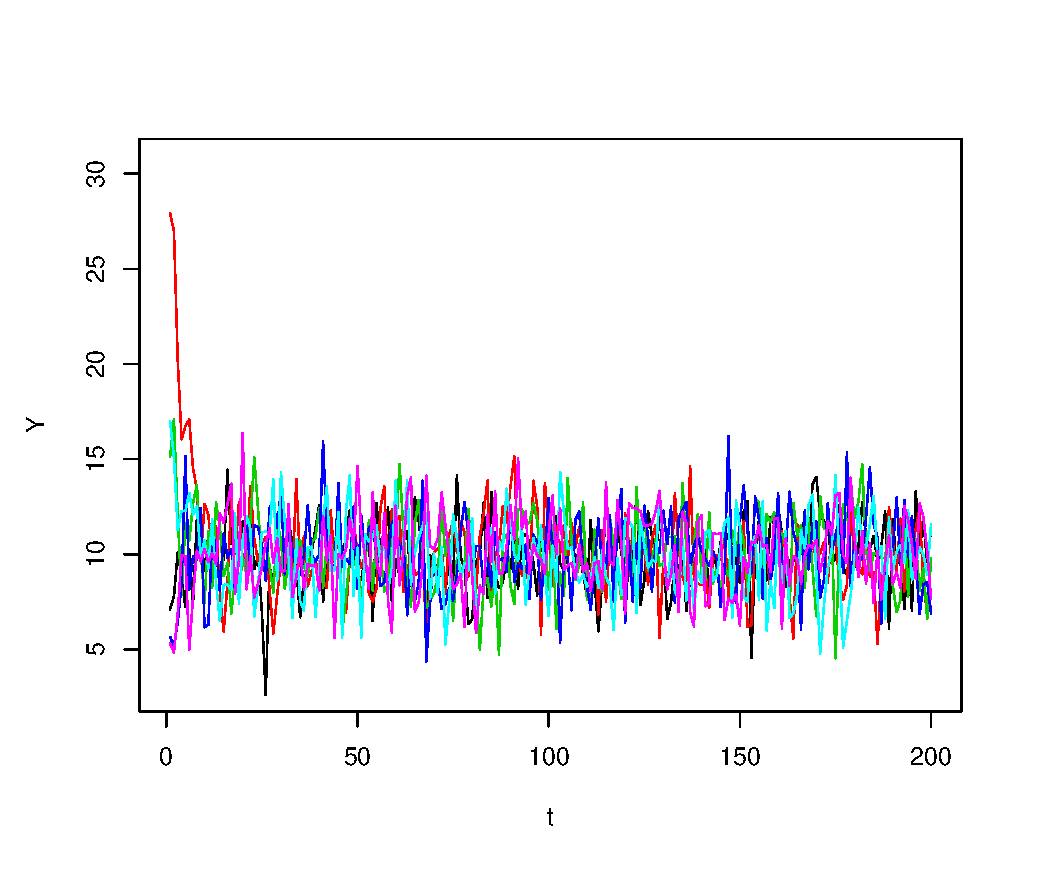
\includegraphics[width = \textwidth]{Model1.eps}
 	\caption{Model 1}
 	\end{subfigure}%
 	\begin{subfigure}[b]{0.45\textwidth}
 	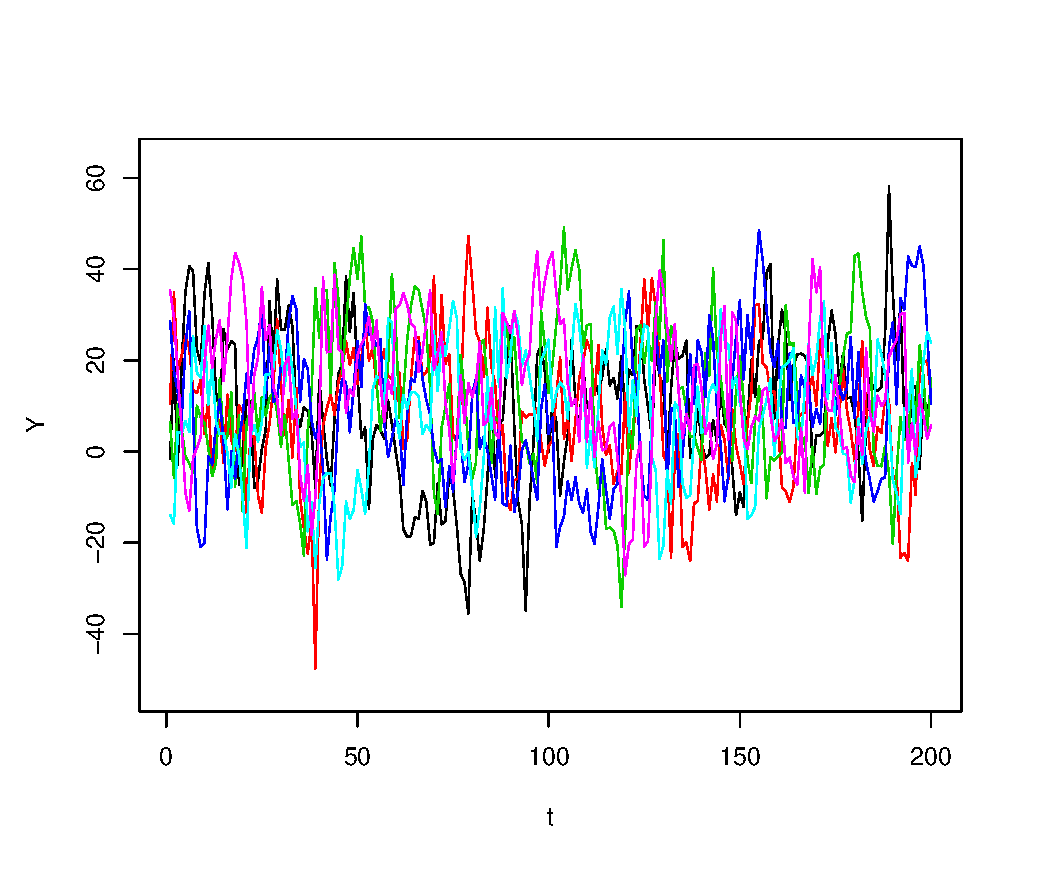
\includegraphics[width = \textwidth]{Model2.eps}
 	\caption{Model 2}
 	\end{subfigure}% 
 	\\
 	\begin{subfigure}[b]{0.45\textwidth}
 	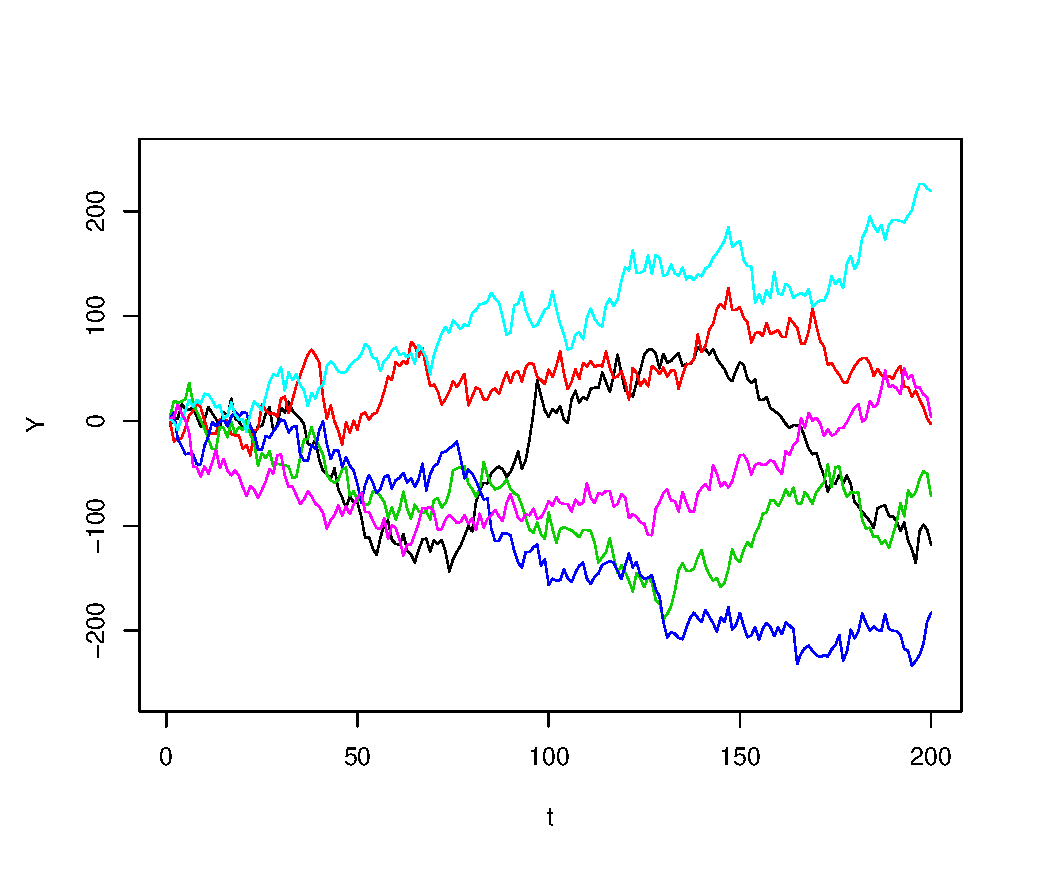
\includegraphics[width = \textwidth]{Model3.eps}
 	\caption{Model 3}
 	\end{subfigure}%
 	\begin{subfigure}[b]{0.45\textwidth}
 	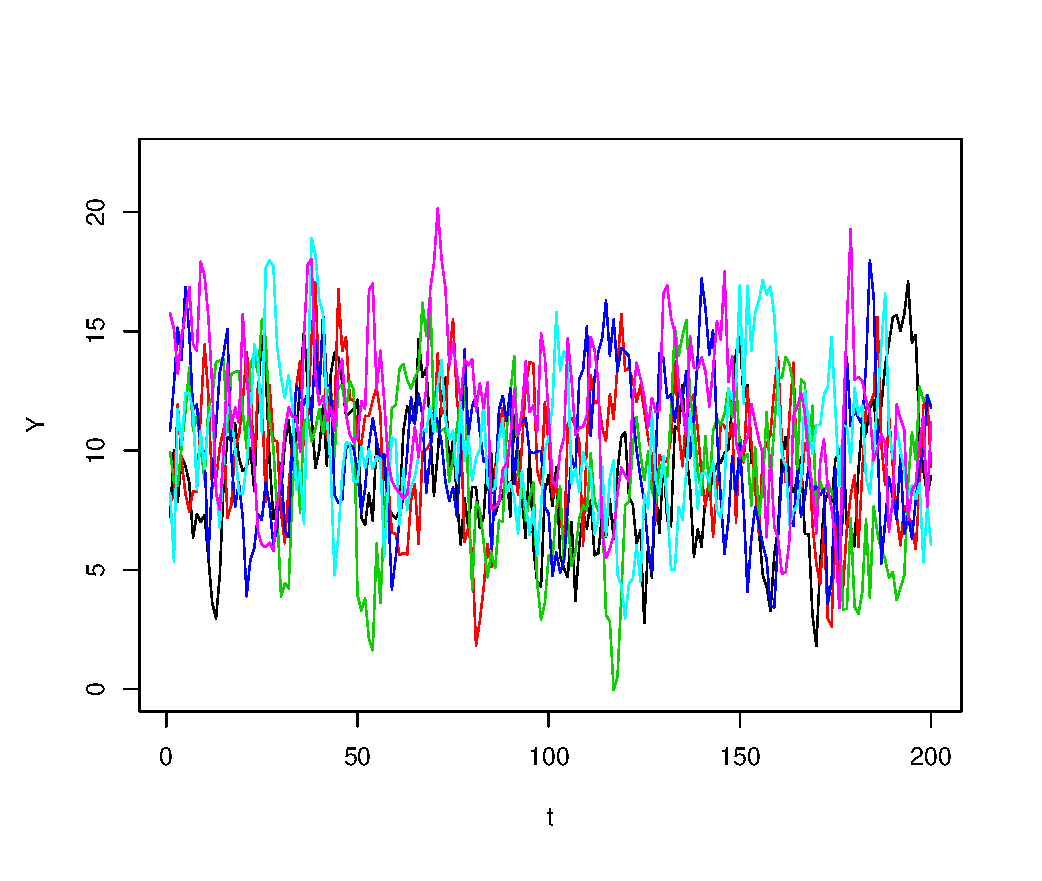
\includegraphics[width = \textwidth]{Model4.eps}
 	\caption{Model 4}
 	\end{subfigure}
 	\caption{$Y(t)$ for 4 models}
 	\label{series}
 \end{figure} 

 \begin{figure}[!htb]
     \centering
 	\begin{subfigure}[b]{0.45\textwidth}
 	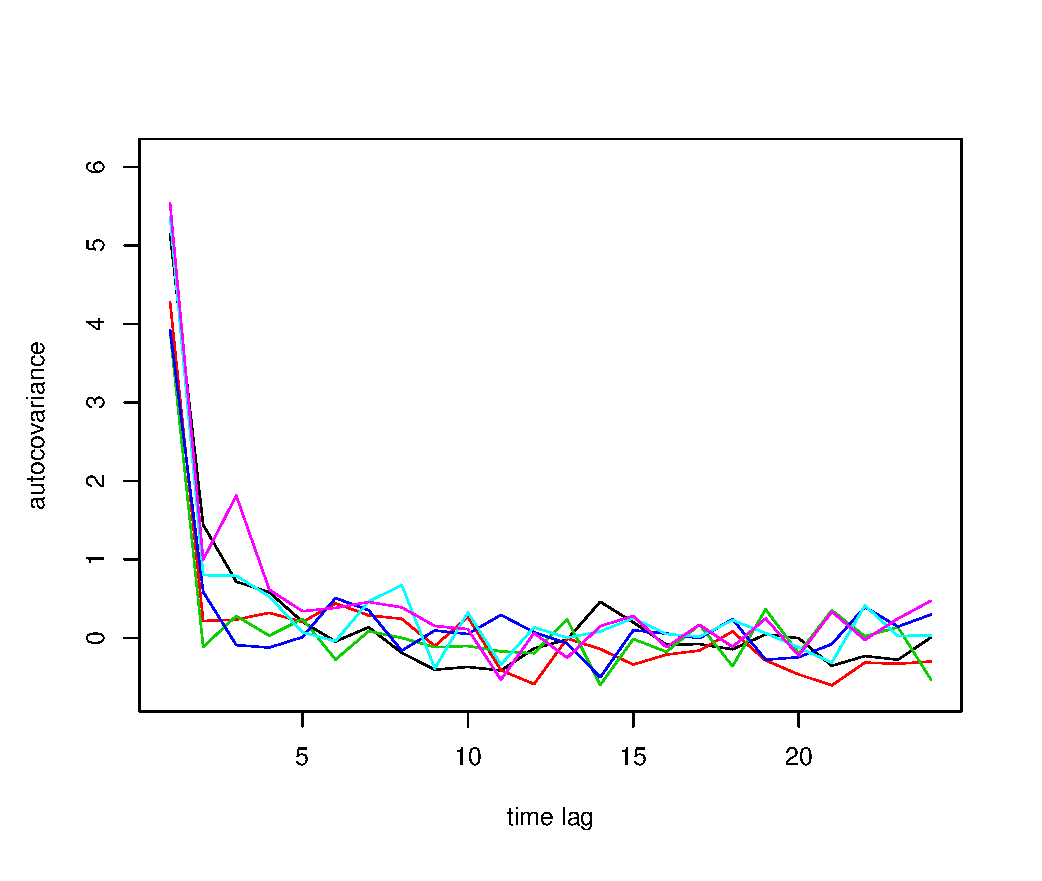
\includegraphics[width = \textwidth]{Model1acv.eps}
 	\caption{Model 1}
 	\end{subfigure}%
 	\begin{subfigure}[b]{0.45\textwidth}
 	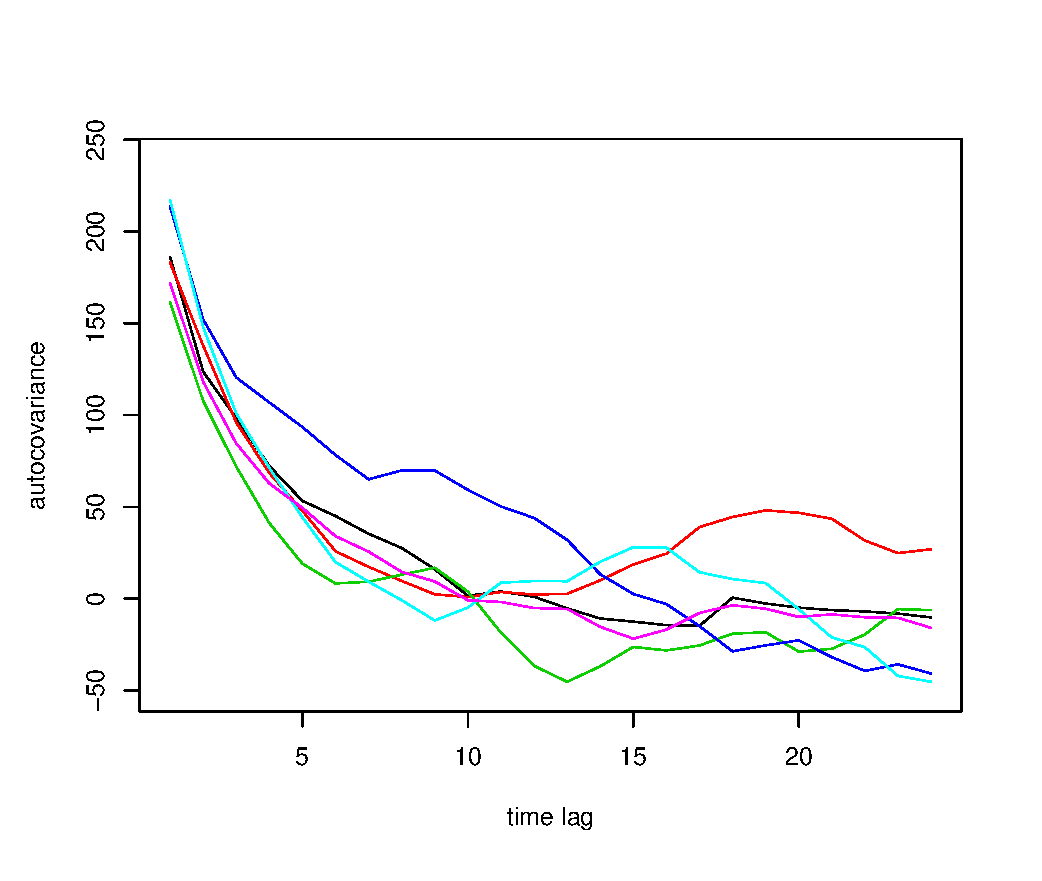
\includegraphics[width = \textwidth]{Model2acv.eps}
 	\caption{Model 2}
 	\end{subfigure}% 
 	\\
 	\begin{subfigure}[b]{0.45\textwidth}
 	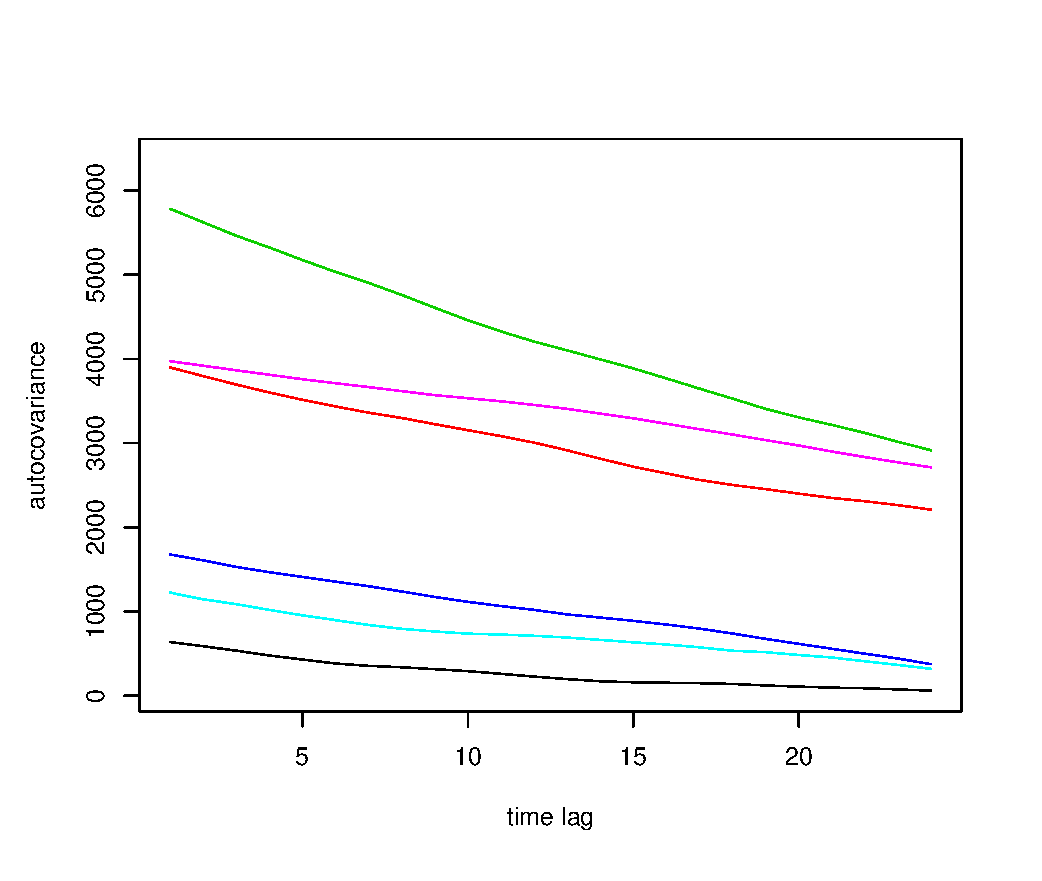
\includegraphics[width = \textwidth]{Model3acv.eps}
 	\caption{Model 3}
 	\end{subfigure}%
 	\begin{subfigure}[b]{0.45\textwidth}
 	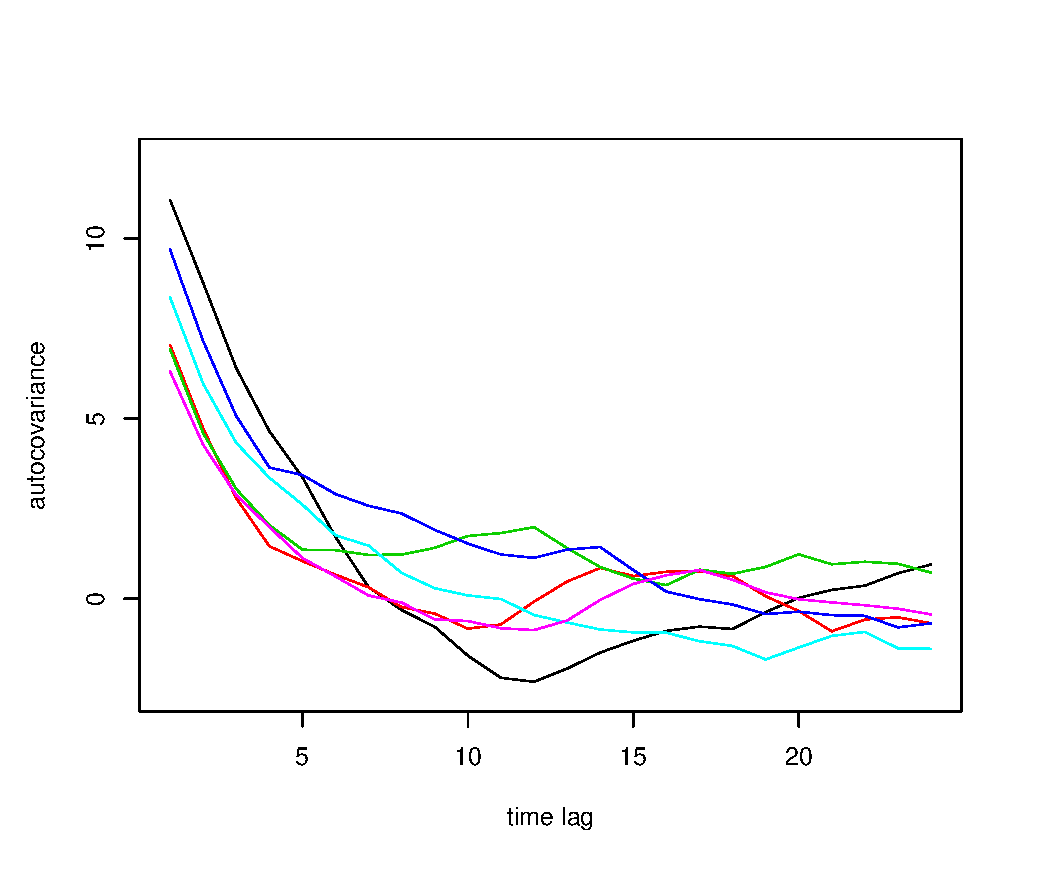
\includegraphics[width = \textwidth]{Model4acv.eps}
 	\caption{Model 4}
 	\end{subfigure}
 	\caption{Sample autocovariance function for 4 models}
 	\label{acv}
 \end{figure} 
 \newpage
 In Figure~\ref{acv} we can see the sample autocovariance also behave pretty much the same for model 2 and model 4 and decreases exponentially. For model 3 the sample autocovariance seems to be decreasing linearly; and for model 1 the sample autocovariance keeps going up and down.  

	











	
	
	
	\end{document}